%######################################## TODO #################################
%############################# Tabulka priorit u SYA ###########################
%################################# Metriky kodu ################################
%################################# Celkova kontrola ############################
\documentclass[12pt,a4paper,titlepage,final]{article}

% cestina a fonty
\usepackage[czech]{babel}
\usepackage[utf8]{inputenc}
% balicky pro odkazy
\usepackage[bookmarksopen,colorlinks,plainpages=false,urlcolor=blue,unicode]{hyperref}
\usepackage{url}
% obrazky
\usepackage[dvipdf]{graphicx}
%\usepackage{svg}	
% velikost stranky
\usepackage[top=3.5cm, left=2.5cm, text={17cm, 24cm}, ignorefoot]{geometry}
\usepackage{indentfirst}

\begin{document}

%%%%%%%%%%%%%%%%%%%%%%%%%%%%%%%%%%%%%%%%%%%%%%%%%%%%%%%%%%%%%%%%%%%%%%%%%%%%%%
% titulní strana

% !!!!!!!!!!!!!!!!!!!!!!!!!!!!!!!!!!!!!!!!!!!!!!!!!
% změň následující údaje za své
\def\author{xxx}
\def\email{xxx@stud.fit.vutbr.cz}
\def\projname{Implementace interpretu imperativního jazyka IFJ14}
% !!!!!!!!!!!!!!!!!!!!!!!!!!!!!!!!!!!!!!!!!!!!!!!!!

\begin{titlepage}

% \vspace*{1cm}
\begin{figure}[!h]
  \centering
  \includegraphics[height=5cm]{img/logo.eps}
\end{figure}

\vfill

\begin{center}
\begin{Large}
Dokumentace k projektu pro předměty IFJ a IAL\\
\end{Large}
\bigskip
\begin{Huge}
\projname\\
\end{Huge}
\begin{large}
Tým XXX, varianta x/x/x\\
\end{large}
\textit{Vedoucí týmu: }\\
\end{center}

\vfill

\begin{center}
\begin{Large}
\today
\end{Large}
\end{center}

\vfill

\begin{flushleft}
%\begin{large}
\begin{tabular}{l l l l l}
\textbf{Řešitelé}: 
&1BIT& Pružina Tomáš, &\url{xpruzi01@stud.fit.vutbr.cz} \\
%Autor: & \author, \url{\email}  \\
% & Fakulta Informačních Technologií \\
% & Vysoké Učení Technické v~Brně \\
\end{tabular}
%\end{large}
\vfill
\begin{large}
Fakulta Informačních Technologií \\
Vysoké Učení Technické v~Brně \\
\end{large}
\end{flushleft}
\end{titlepage}


%%%%%%%%%%%%%%%%%%%%%%%%%%%%%%%%%%%%%%%%%%%%%%%%%%%%%%%%%%%%%%%%%%%%%%%%%%%%%%
% obsah
\pagestyle{plain}
\pagenumbering{roman}
\setcounter{page}{1}
\tableofcontents

%%%%%%%%%%%%%%%%%%%%%%%%%%%%%%%%%%%%%%%%%%%%%%%%%%%%%%%%%%%%%%%%%%%%%%%%%%%%%%
% textova zprava
\newpage
\pagestyle{plain}
\pagenumbering{arabic}
\setcounter{page}{1}

%%%%%%%%%%%%%%%%%%%%%%%%%%%%%%%%%%%%%%%%%%%%%%%%%%%%%%%%%%%%%%%%%%%%%%%%%%%%%%
\section{Úvod} \label{uvod}
%=============================================================================
Implementace překladače imperativního jazyka je netriviální úloha, proto je
vhodné ji rozdělit na podúlohy (\ref{moduly_interpretu}), které jsou vhodně
rozdělené mezi členy týmu, který je vedené a kontrolován týmovým vedoucím.

Tento dokument se skládá z N částí, které popisují jednotlivé moduly
interpretu imperativního jazyka IFJ14, a to jsou lexikální analyzátor
(\ref{lexikalni_analyzator}), syntaktický analyzátor (\ref{syntakticky_analyzator})
využívající rekurzivní sestup (), který je pro potřeby syntaktické
analýzy výrazů rozšířený o Shunting-Yard (\ref{sya}) algoritmus\footnote{Byla nám
dovolena výjimka, implementovat a náležitě zdokumentovat tento algoritmus oproti předepsané
precedenční analýze}. Kontrola syntaxe a sémantiky probíhá z velké části při jednom
průchodu, následné kontroly sémantiky probíhají až za běhu.

Jelikož je projekt založen na týmové spolupráci, rozhodli jsme se využít možnosti používat verzovacího systému, jmenovitě \verb|bitbucket|. Vzhledem k tomu, že práce byla rozdělena mezi jednotlivé členy a probíhaly kontroly v době schůzek, jevil se tento systém jako nejlepší, do jisté míry totiž umožňuje porovnávání verzí a tím se dá kontrolovat, zdali daný člen splnil svou část úkolu či nikoliv.

Práce v týmu byla rozdělena následovně: \textbf{Martin Juřík} měl na starost zpracování lexikálního analyzátoru a jeho funkční otestování. Dále pak parser a tedy syntaktickou a sémantickou část projektu vytvářel \textbf{Antonín Marko}. Návrh a vytvoření interpretu dostal na starosti \textbf{Tomáš Pružina}. Celkové testování, zpracování LL gramatiky a dokumentaci měl na starosti \textbf{Martin Kubíček}. \textbf{Petr David} úprava knihovních funkcí a vestavěné funkce do předmětu \verb|Algoritmy|.

Za účelem testování a ověření plné funkčnosti projektu byla napsána sada testů, obsahující i vlastní testovací skript, čítající zhruba \textbf{8} odvětví s celkovým počtem \textbf{362} testů. Úkolem testování, bylo především schopnost odchytávat všechny možné chyby, které by mohly nastat a vracení správného chybového kódu. Ovšem ne vždy bylo určení správného chybového kódu jednoduché, jelikož jsme narazili na pár sporných momentů, které jsme se snažili vyřešit důkladnějším studiem dokumentace k projektu nebo společnou debatou v týmu. Dále jsme testy ověřovaly do jaké míry, jsme schopni správně interpretovat validní data.

%%%%%%%%%%%%%%%%%%%%%%%%%%%%%%%%%%%%%%%%%%%%%%%%%%%%%%%%%%%%%%%%%%%%%%%%%%%%%%
\section{Moduly interpretu jazyka} \label{moduly_interpretu}
%=============================================================================
\subsection{Lexikální analyzátor} \label{lexikalni_analyzator}

Syntaktický analyzátor potřebuje ke své činnosti lexikální analyzátor. Ten
předává na žádost syntaktického analyzátoru tzv. tokeny, které získává postupným
čtením vstupního souboru, který obsahuje zdrojový kód napsaný v jazyce IFJ14.
Samotný výsledný token je reprezentací lexému (identifikátor, klíčové slovo,
příkaz přiřazení atp.).

Pro úspěšné rozlišení typu lexému se v naší implementaci používá konečný
automat, jehož struktura je znázorněna na obrázku (\ref{lex_ka}).

Jestliže se konečný automat v době zpracovávání řetězce zdrojového souboru
dokument do chybového stavu \verb|lexerrref|, řetězec je nepřijatý a jedná se
o lexikální chybu. Samotná implementace lexikálního analyzátoru patří k
jednodušším částem projektu, avšak jeho návrh a testování zabralo nemálo času.

%<insert KA diagram here>
\begin{figure}[h!]\label{lex_ka}
	\centering
		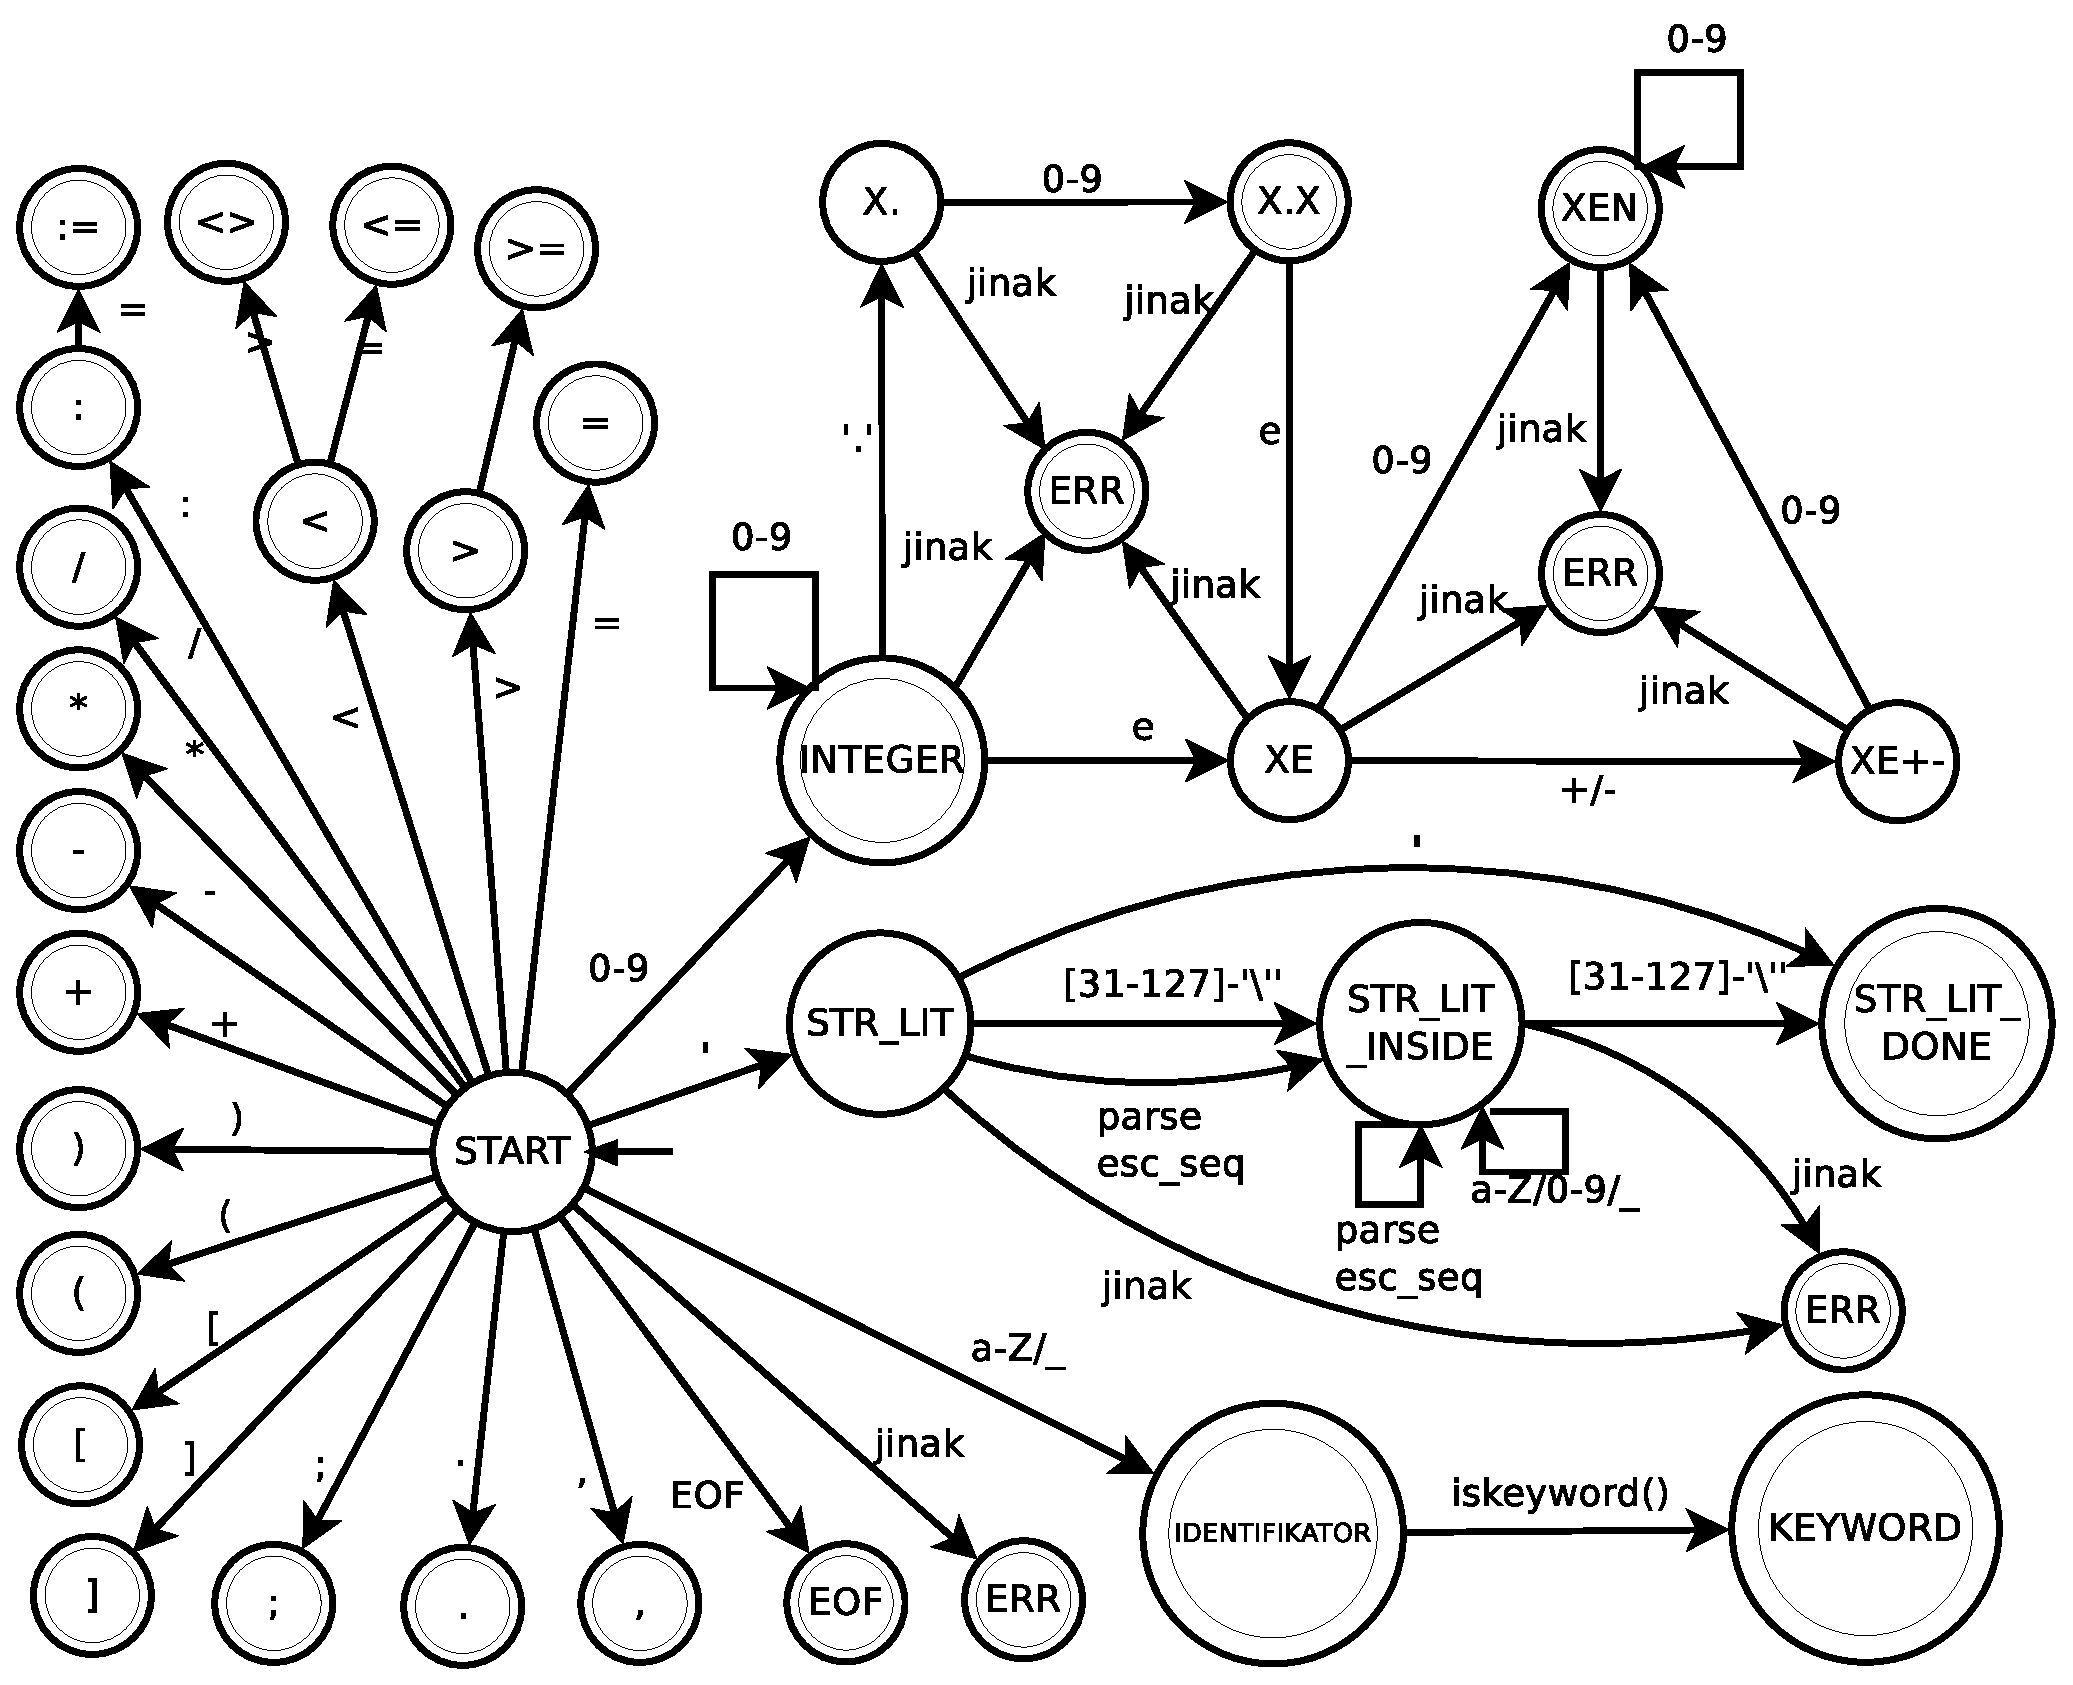
\includegraphics[width=\textwidth]{img/KA-scanner.eps}
	\caption{Konečný automat lexikálního analyzátoru}
\end{figure}
\pagebreak

\subsection{Syntaktický analyzátor} \label{syntakticky_analyzator}
Jak již bylo zmíněno, syntaktický analyzátor žádá lexikální analyzátor o tokeny
a na základě sekvence po sobě jdoucích tokenů sestavuje abstraktní syntaktický
strom (dále jen AST). Tato sekvence musí odpovídat pravidlům syntaxe jazyka IFJ14,
v opačném případě se jedná o syntaktickou chybu.

Jazyk IFJ14 je staticky typovaný jazyk, tedy typové kontroly probíhají během 
překladu, v našem případě právě při průchodu syntaktickým analyzátorem. Je tedy
nutné zachytávat chybové vstupy a přímo ukončovat průchod a tím i celou aplikaci.

Jako vnitřní kód programu jsme si zvolili AST, tedy binární strom a rozšířili jsme
jeho strukturu o potřebné položky pro práci interpretu. Jak již bylo zmíněno výše,
jedná se o binární strom, má tedy dva synovské uzly. Avšak pro určité typy uzlů
je mít nemusí. Například uzel pro operaci \verb|NOT| má pouze levý synovský podstrom.

Pro převod příkazů obsahujících tělo na AST uzly byla v týmu domluvena konvence,
že primárním uzlem pro tělo bude levý podstrom. Tedy například cyklus \verb|while|
má svoje tělo uložené v levém podstromu. Zde je potřeba zmínit, že příkaz \verb|if|
má v podstatě dvě sekvence příkazů a to pravdivou a nepravdivou. Je tedy potřeba
zajistit, aby se obě uchovaly v jednom uzlu AST.

Řešení je jednoduché a více než samozřejmé, uložení pravdivé sekce do levého
poduzlu stromu a nepravdivou sekci do uzlu pravého. U příkazů s podmíněným
chováním (if, while, repeat-until, atp.) bylo nutné uchovat podmínku, tedy výraz,
který určuje, jestli je příkaz proveditelný či není. Primárně pro tento účel
slouží dodatečná položka uzlů AST, která svým typem \verb|void*| umožňuje
mnohostranné využití. 

Zvláštní případ použití dodatečné položky je například u definice či volání funkce.
V tomto případě obsahuje strukturu \verb|String| se jménem funkce. Levý podstrom
opět obsahuje tělo funkce a v pravém podstromu je uložen uzel se strukturou \verb|varspars|,
která se složená z dvou front, jedné pro lokální proměnné funkce a druhá pro
parametry funkce. Tyto fronty jsou naplněny při definici funkce, při deklaraci
(použití \verb|forward| deklarace) je naplněna pouze fronta parametrů. Více o funkcích
v \ref{func}.

\subsubsection{Shunting-yard algoritmus}
\label{sya}
Pro zpracování výrazu mělo být původně v projektu užito precedenční analýzy. My jsme ovšem toto zpracování řešili pomocí Shunting-yard algoritmu\footnote{Byla nám
dovolena výjimka, implementovat a náležitě zdokumentovat tento algoritmus oproti předepsané
precedenční analýze}. Algoritmus zpracování výrazů je založen na prioritě operátorů, které buď vkládá
nebo odebírá ze zásobníku a vkládá do výstupní sekvence. Tento algoritmus primárně
slouží k převodu infixového zápisu výrazů do postfixového, tedy lépe zpracovatelného
a převeditelného do AST.

Tento algoritmus byl pro potřeby projektu upraven, aby přímo generoval AST místo
výstupního postfixového zápisu a zároveň u tvorby jednotlivých uzlů zastupujících
operace kontroloval, zdali datový typ vrcholových uzlů synovských uzlů odpovídá
sémantickým pravidlům zpracovávání výrazů. Což nám poskytuje možnost pouze jediného průchodu, který tak stačí na zpracování.

Toto řešení ovšem není tak přínosné jak se zdálo, jelikož při tvorbě výrazů je nutné kontrolovat spoustu aspektů validního výrazu. To jsou
například datové typy jednotlivých operandů v případě binárních operací.

\subsection{Interpret} \label{interpret}

Interpret je závěrečnou částí projektu. Rekurzivně zpracovává AST reprezentovaný
binárním stromem a postupně vykonává operace nad ním definované.

Kořenem tohoto AST je vždy typ převedené operace, přičemž obsahuje předem
definované nepovinné parametry (příkladem je podstrom volání funkce, který
obsahuje předávání proměnné). Tedy každý uzel AST představuje jednu atomickou
operaci, kterou je řízený samotný běh programu.

Interpret samozřejmě nepracuje jen se samotným syntaktickým stromem, ale
taktéž s tabulkou symbolů, která obsahuje data potřebná na to, aby interpret
mohl vykonávat nějakou užitečnou práci definovanou v těle programu.

Interpret tedy spravuje tabulky symbolů, dynamicky je za běhu
vykonávaného programu vytváří a (podle potřeby) ruší.

V neposlední řadě interpret vykonává sémantickou kontrolu u operacích, které
syntaktický analyzátor v době zpracování vstupního programu a generování
abstraktního syntaktického stromu neřešil.

Příkladem takovéto kontroly je používání (čtení) proměnné před její řádnou
definicí (přiřazením hodnoty) anebo dělení nulou v aritmetickém výrazu.

Takovéto běhové chyby jsou v interpretu řešené ukončením interpretace a navrácením
chybového kódu podle zadání imperativního jazyka IFJ14.

\subsubsection{Tabulka symbolů} \label{tabulka_symbolu}

Tabulka symbolů je implementována pomocí binárního vyhledávacího stromu,
přičemž se rozlišuje několik úrovní tabulky symbolů.

Každý program obsahuje globální tabulku symbolů (ve které jsou uložené ukazatele
na funkce) a lokální tabulku symbolů, která obsahuje běhové proměnné
vykonávaného programu.

Z implementačního hlediska jsou lokální tabulky symbolů (stromy) ukládané na
zásobník, přičemž platí, že při volání funkce se vytvoří nová (lokální)
tabulka symbolů, do které se zkopírují příslušné parametry volané funkce z
nižší vrstvy lokální tabulky (popř. z globální tabulky symbolů).

Taková lokální tabulka taktéž obsahuje návratovou hodnotu vykonávané funkce,
která umožňuje rekurzivní volání funkcí a samozřejmě umožňuje vykonávat tělo
funkce bez nutnosti jakkoliv zasahovat do abstraktního syntaktického stromu.


%%%%%%%%%%%%%%%%%%%%%%%%%%%%%%%%%%%%%%%%%%%%%%%%%%%%%%%%%%%%%%%%%%%%%%%%%%%%%%
\section{Postup při implementaci řešení} \label{postup_pri_implementaci_reseni}
%=============================================================================
\subsection{Funkce \texttt{sort}}
K implementaci funkce sort jsme podle zadání použili algoritmus quicksort.
Kromě funkce quicksort jsme potřebovali ještě pomocnou funkci \verb|partition|,
která rozděluje řazené pole na dvě části. V jedné takto vzniklé části jsou prvky
s menší hodnotou než je prvek rozdělující tyto části (pseudomedián, dále jen PM)
a v druhé části prvky s hodnotou větší než PM. Index PM určíme jako $(l+p)/2$, kde
$i$ je index nejlevějšího prvku řazeného úseku pole a $j$ index nejpravějšího prvku
tohoto pole. Všechny prvky s hodnotou nižší než je PM poté přesuneme na levou
stranu od PM a prvky s vyšší hodnotou na pravou stranu. Poté aplikujeme algoritmus
quicksort na obě poloviny pole.

Konkrétní implementace algoritmu je převzata z přednášek předmětu Algoritmy
(IAL2014 \cite{honzik2} -- 10. přednáška 33. slide). Pro snazší konverzi do jazyka
C a pro pochopení algoritmu samotného jsme vytvořili vývojový graf a podle grafu
jsme sepsali samotný kód v jazyce C.

\paragraph{Modifikace:} Algoritmus popsaný v přednáškách obsahoval prohození
prvku se sebou samým, takže jsme provedli drobnou úpravu, která tomuto zabránila.

\subsection{Funkce \texttt{find}}
Pro funkci find jsme dle zadání použili KMP (Knuth-Morris-Prattův algoritmus).
Jedná se o algoritmus využívající konečný automat. Tento konečný automat využívá
hrany ANO/NE. Nejprve bylo nutné vytvořit si pole \verb|FAIL|, do kterého se
uloží zjištěné hodnoty posunů. Poté přijde na řadu samotné vyhledávání řetězce.
Nejprve zarovnáme podřetězec a řetězec na první index. Pak se jen porovnávají znaky,
pokud jsou shodné, zvyšuje se index o 1 v podřetězci, který hledáme (\verb|pattern|)
a zároveň i v řetězci, ve kterém vyhledáváme (\verb|text|). Pokud nikoliv, tak se
vracím po hraně "N" (NE hrana) neboli \verb|FAIL| vektor. Je-li pak hodnota indexu
v hledaném řetězci rovna délce hledaného podřetězce, tak byl nalezen vzorek na
indexu $TInd - PL$, kde $TInd$ je index řetězce a $PL$ je délka hledaného podřetězce,
jinak nic nenašel a vrací se 0.

Algoritmus byl převzán a přepsán do jazyka C z přednášek předmětu Algoritmy (IAL2014
\cite{honzik2} -- 11. přednáška 18. slide).
 
\paragraph{Modifikace:} Pro návrat 0 v případě neúspěchu byla provedena modifikace
algoritmu z přednášek, kde byl vracen poslední dosažený index, tedy délka řetězce.

\subsection{Funkce \texttt{copy}}
Umožňuje kopírovat hodnotu ze zadaného stringu, do nového. K vytvoření nového stringu složí funkce \verb|makeNewString|, která je podrobně popsána v knihovně \verb|string.c|, který zajišťuje práci s řetězci. Avšak před samotným uložením se provedou sady kontrol. Jako například zda předávaná hodnota či celá struktura nejsou nulové, jestli počáteční index odpovídá hodnotě 0 tedy standardu C-like a v poslední řadě, zda délka není menší či rovna 0. Po samotné alokaci paměti pro daný string se upraví indexování, aby odpovídalo C-like standardu. Jelikož, je použit implementační jazyk C, který neumí pracovat se stringy je zde string interpretován jako posloupnost za sebou jdoucích znaků typu char uložených do pole.

\subsection{\texttt{Shunting-yard algoritmus}}
Jak už bylo výše zmíněno algoritmus funguje na bázi priority, kde v našem případě jsou priority stanoveny takto(bráno od nejvyšší po nejnižší, je zda zahrnuto i rozšíření):[not], [Logický and, násobení, dělení], [sčítání, odčítání, or, xor], [porovnávací operátory] pokud se zde objeví něco jiného je nahlášena chyba. Konkrétně je algoritmus implementován jako funkce \verb|parseExpression| v \verb|parser.c|. Obsahuje jeden nekonečný cyklus, který se ukončí pouze v případě chyby či ukončení výrazu. Zpracování obsluhuje jeden obsáhlý switch, který se snaží pokrýt všechny možné situace, poté provede příslušené úkony dle toho jaká část výrazu právě zpracovává. Největší problémem zde bylo odchytáváním specifických chyb. Např.: \verb|(3(+8))|, která je řešena tak, že pokud načteme levou závorku, uschováme si ji a pokud za ní následuje operátor je vypsána příslušná chyba.

\subsection{Rozšíření}
\subsubsection{Array}
Díky tomu, že je potřebné, vždy předdefinovat pole bude se nejdřív tato definice ukládat do stromu, kde se vytvoří uzel \verb|AST_ARR| a jeho synovské uzly budou prázdné (tedy budou sloužit k provázání stromu) a datová struktura bude obsahovat jméno dané proměnné. Do položky other se uloží \verb|dataTypeArray| struktura, ve které jsou uloženy informace o rozsahu pole. Strukturu potom zkopírujeme odkazem i do indexovacího uzlu, který má v levém synovském uzlu \verb|AST_ID| a v pravem \verb|AST_INT|, protože indexovat se může pouze celočíselným literálem.
\subsubsection{Repeat}
Pro interpretaci Repeatu jsme použili už vytvořenou funkci pro parsování While ovšem s tou změnou, že jsme obrátili parsováním, tedy nejdřív musíme zpracovat tělo a poté až podmínku. Jelikož v zadání stojí, že Repeat nemusí disponovat tělem, tedy nemusí obsahovat begin a end, museli jsme udělat další změnu a mohli jsme tedy vypustit podmínku, která obsahovala klíčová slova begin a end.
\subsubsection{ElseIf}
K zhotovení tohoto rozšíření stačilo pouze více rozvést funkci na zpracování podmínky IF a zahrnout do ní možnosti, které pokrývá toto rozšíření.
\subsubsection{BoolOp}
Jelikož se Boolovské operátory využívají ve výrazech, byla nutná změna především Shunting-yard algoritmu, do kterého jsme museli implementovat nové priority. Přesněji jsme museli přidat prvek s nejvyšší prioritou čímž je NOT, další priority jsou pak na stejné úrovni jako v původním Shunting-yard algoritmu.
\subsubsection{For}
For umožňuje dvě možnosti interpretace a to inkrementální a dekrementační, což přináší jisté komplikace. Tělo cyklu bude v levém poduzlu typu \verb|AST_FOR|, v pravém poduzlu bude podmínka. Pokud bude, cyklus for v inkrementační verzi uloží se typ vrcholu jako \verb|AST_FOR_TO| v opačném případě se tam vloží typ \verb|AST_FOR_DOWNTO|.

\section{LL-tabulka} \label{lltabulka}
Uvedená LL - tabulka je zpracována pouze pro zakladní zadaní bez rozšíření.
\begin{verbatim}
PROGRAM         -> VARS FUNC begin CMD_LIST enddot

VARS            -> var VAR_DEF VAR_DEFS
VARS            -> eps
VAR_DEFS        -> VAR_DEF VAR_DEFS
VAR_DEFS        -> eps
VAR_DEF         -> id : DT_TYPE ;

DT_TYPE         -> integer
DT_TYPE         -> real
DT_TYPE         -> boolean
DT_TYPE         -> string

FUNC            -> eps
FUNC            -> HEADER

HEADER          -> function id ( DEF_PARAMS ) : DT_TYPE ; AFTER_HEADER

AFTER_HEADER    -> forward ;
AFTER_HEADER    -> VARS BODY ;

DEF_PARAMS      -> eps
DEF_PARAMS      -> DEF_PAR DEF_PAR_LIST

DEF_PAR_LIST    -> eps
DEF_PAR_LIST    -> ; DEF_PAR

DEF_PAR         -> id : DT_TYPE

BODYN           -> begin CMD_LIST_N end
CMD_LIST_N      -> eps
CMD_LIST_N      -> CMD CMD_FOLLOW
CMD_FOLLOW      -> eps
CMD_FOLLOW      -> ; CMD CMD_FOLLOW

BODY            -> begin CMD_LIST end
CMD_LIST        -> CMD CMD_FOLLOW

CMD             -> ASSIGN
CMD             -> BODYN
CMD             -> IF
CMD             -> WHILE
CMD             -> WRITE
CMD             -> READLN

ASSIGN          -> id := AFTER_ASSIGN
AFTER_ASSIGN    -> EXPR
AFTER_ASSIGN    -> CALL

IF              -> if EXPR then BODYN IF_ELSE
IF_ELSE         -> eps
IF_ELSE         -> else BODYN
WHILE           -> while EXPR do BODYN

CALL            -> id ( TERM_LIST )
CALL            -> sort ( dt_str )
CALL            -> find ( dt_str , dt_str )
CALL            -> length ( dt_str )
CALL            -> copy ( dt_str , dt_str , dt_int )

READLN          -> readln ( id )
WRIT            -> write ( TERM_LIST )

TERM_LIST       -> TERM
TERM_FOLLOW     -> , TERM TERM_FOLLOW
TERM_FOLLOW     -> eps

TERM            -> id
TERM            -> dt_int
TERM            -> dt_real
TERM            -> dt_bool
TERM            -> dt_str

EXPR            -> vyraz
\end{verbatim}
\pagebreak
%%%%%%%%%%%%%%%%%%%%%%%%%%%%%%%%%%%%%%%%%%%%%%%%%%%%%%%%%%%%%%%%%%%%%%%%%%%%%%
\section{Závěr} \label{zaver}
Jelikož většina lidí z týmu projekt opakuje, snažili jsme se vše zhotovit s předstihem a s co nejvíce možnými rozšířeními. Ovšem opět nás zaskočila časová náročnost projektu a také hlavně jeho rozsáhlost. Občas jsme měli i problémy s rozdílností interpretovaných jazyků a museli jsme náš původní návrh, který vznikal ještě na samém začátku semestru a z poznatků z minulého roku, mnohokrát upravovat. Avšak díky velké sadě testovacích skriptů jsme byli schopni otestovat většinu možných situací a podchytit tak dost chyb.
%%%%%%%%%%%%%%%%%%%%%%%%%%%%%%%%%%%%%%%%%%%%%%%%%%%%%%%%%%%%%%%%%%%%%%%%%%%%%

\appendix

\section{Metriky kódu} \label{metriky}
Počet všech zdrojových souborů: 21

celkový počet řádků: 

Velikost spustitelného programu (bez debugovacích informací, Gento 64bit): bytů

Velikost spustitelného programu (bez debugovacích informací, Ubuntu 64bit): bytů


%%%%%%%%%%%%%%%%%%%%%%%%%%%%%%%%%%%%%%%%%%%%%%%%%%%%%%%%%%%%%%%%%%%%%%%%%%%%%%
% seznam citované literatury: každá položka je definována příkazem
% \bibitem{xyz}, kde xyz je identifikátor citace (v textu použij: \cite{xyz})
\begin{thebibliography}{1}

% jedna citace:
\bibitem{honzik}
HONZÍK J. M.: \emph{Studijní opora pro předmět Algoritmy}. Elektronický text. FIT VUT v Brně
\bibitem{honzik2}
HONZÍK J. M.: \emph{Přednášky k předmětu Algoritmy}. Soubor elektronických textů. FIT VUT v Brně
\bibitem{meduna}
MEDUNA A., LUKÁŠ R., \emph{Podklady k přednáškám}. Elektronický text. FIT VUT v Brně
\bibitem{meduna2}
MEDUNA A., LUKÁŠ R., \emph{Studijní opora pro předmět Formální jazyky a překladače}. Elektronický text. FIT VUT v Brně


\end{thebibliography}
%%%%%%%%%%%%%%%%%%%%%%%%%%%%%%%%%%%%%%%%%%%%%%%%%%%%%%%%%%%%%%%%%%%%%%%%%%%%%%
\appendix

\end{document}